
\subsection{Executed Attacks} 

We demonstrated several attacks on various controllers utilizing our rogue switch utility. 
   
\subsubsection{Dropping traffic}
The rogue switch could simply drop packets sent to it, thus creating a service interruption. However, a controller would probably notice this quickly -- it would appear as though the switch had failed, and automated recovery mechanisms would be initiated.

\subsubsection{Cloning or diverting traffic}
A compromised switch could ensure that traffic would be routed through an adversary's middlebox, or could clone traffic and send the cloned stream to the adversary. This would be more difficult for the controller to detect, unless it caused considerable slowdown. This attack could conceivably be used for purposes such as the NSA's MUSCULAR program, which intercepts traffic as it flows between private data centers \cite{muscular}. 

\subsubsection{DOS on the Controller}
We utilized the basic layer 2 MAC address learning example from each controller with a modified the hard flow timeout of 1 as our setup\footnote{We used l2\_learning as our Pox controller and l2\_switch as our Ryu controller.}. We also utilize the basic mininet setup (1 switch with 2 hosts) to test the delay caused by our attack on each controller. To test the delay cause on the controller, we would simply have h1 ping h2. A more complicated controller (e.g. one that does more than simply add the mac address as a flow) would see its performance decrease more significantly than in our example test cases.

 The first attack we attempted was to see if a single switch could overload the controller by rapidly pushing information. We utilized the basic Echo Request (the switch keep-a-live message) as the OpenFlow message to send to the controller to establish a baseline for testing. Bigger packets, particularly ones that require some sort of computation by the controller application, would increase the performance effect on the controller. We started by sending a Echo Request as quickly as possible to the controller without caring about the response. This attack had little effect of the controller and simply resulted in periodic "TCP Previous Segment Lost" messages as a response from the controller. We believe that the issue with this method was we were never reading in the Echo Replies sent from the controller and the controller was simply ignoring our messages because its send buffer was full. We then modified this attack to send a single Echo Request, wait for an Echo Reply and then instantly send another. This attack caused the controller to continually send Echo Replies but at a controller specified rate - we had to wait for a reply before sending another request. As a result, this attack also had little effect on the controller.

\begin{figure}
  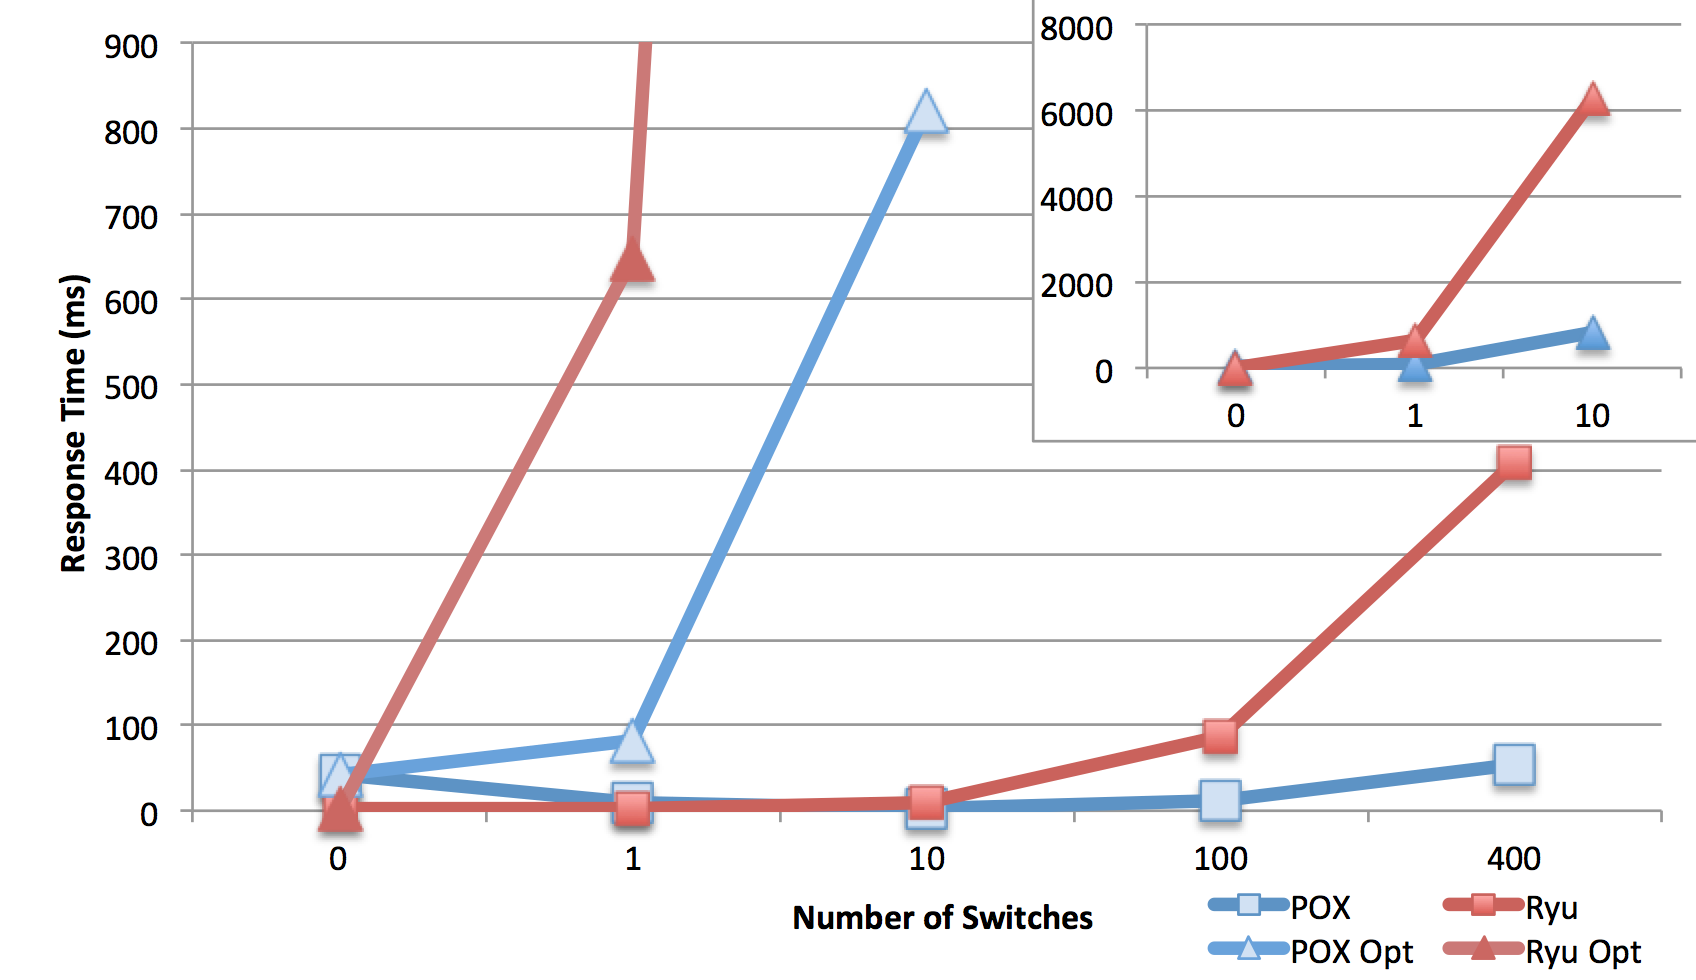
\includegraphics[width=\linewidth]{DOSAttack.png}
  \caption{Results of DOS Attacks on the Controller \cite{protocol}}
  \label{fig:DOSattacks}
\end{figure}

\subsubsection{DDoS on the Controller}
   To increase the effect of our attack, we created multiple rogue switches and had each utilize the same attack on the controller. Our testing machine was actually the limiting factor in the number of rogue switches we could spawn, but we utilized 400 switches as the max for comparison purposes.  We further optimized our attack by splitting our TCP socket into a distinct listener and sender. We threaded our application so the two actions were not dependent on each other and achieved significantly better results. With out optimized version, we were able to push packets fast enough to cause TCP Window Zero Errors and the controller to have to drop packets.  These results (shown in Figure 2) show that even a single switch can severally effect the performance of a controller and therefore degrade an entire network. 

\subsection{Other Possible Attacks}
\subsubsection{DoS other switches}
By injecting traffic, a switch could deliberately attempt to overload neighboring switches' TCAMs or otherwise DoS them. The rogue switch could leverage its connection to the controller in order to prompt the controller to broadcast many erroneous flow modifications; thus, instead of attacking each network element individually, the controller gives the attacker an easy, cheap way to concurrently many switches at once. 

\subsubsection{Advertising false host attachments}
A rogue switch could send the controller packet-in events with false packets, which falsely claim to have a particular MAC address attached to them. This could lead the controller to believe that the compromised switch should receive traffic intended for the host. While this would soon lead to packet loss and a noticeable disruption, it would nevertheless allow a switch to eavesdrop when it would not normally be in a position to do so.

\subsubsection{Falsify measurement reports}
A switch may return false results in response to a read-state  measurement message, thus causing the controller to behave irrationally. For example, a switch could falsify or hide a DoS attack, elephant flows, etc.

\subsubsection{Ignoring rules}
A compromised switch could initially imitate a normal switch, so that it receives traffic and operates as a part of the network, and then selectively ignore flow-table modification requests. For example, dropping packets will be noticed quickly; but a switch could allow packets to pass through that should have been dropped. Because of the difficulty of querying flow table state, the controller may not become aware of this. A compromised switch could thus operate in ``stealth mode" and the inconsistent flow table might only be noticed once the switch allows an attacker to pass through, for example.

\subsubsection{Modifying VLAN tags}
A switch could modify VLAN tags in order to have malicious traffic be erroneously treated by other network elements. For example, if normal only packets with a certain VLAN tag are allowed to access a sensitive resource, the switch could ensure that the attacker's traffic appears to have valid permissions. % I'm really not so sure about this one, so maybe we shouldn't include it.

\subsubsection{Reporting flow mods to an adversary}
An adversary could hope to learn about network traffic by observing flow mods. Certain flow mods might indicate that the controller has, for example, detected an intrusion, or that a specific host has connected to the network in a certain location. Thus, just knowing what flow mods are being issued by the controller could be a source of interesting information for an adversary.

\subsubsection{Fingerprinting controller applications}
Similarly, the rogue switch could send packets directly to the controller and observe the controller's response in order to determine what kinds of applications are probably running on the controller. This information could then be used by an attacker to more narrowly target future attacks.
